\begin{frame}[plain, c]
    \centering
    \vspace{5em}
    \Huge
    Agentic AI
\end{frame}


\begin{frame}{}
  \centering
  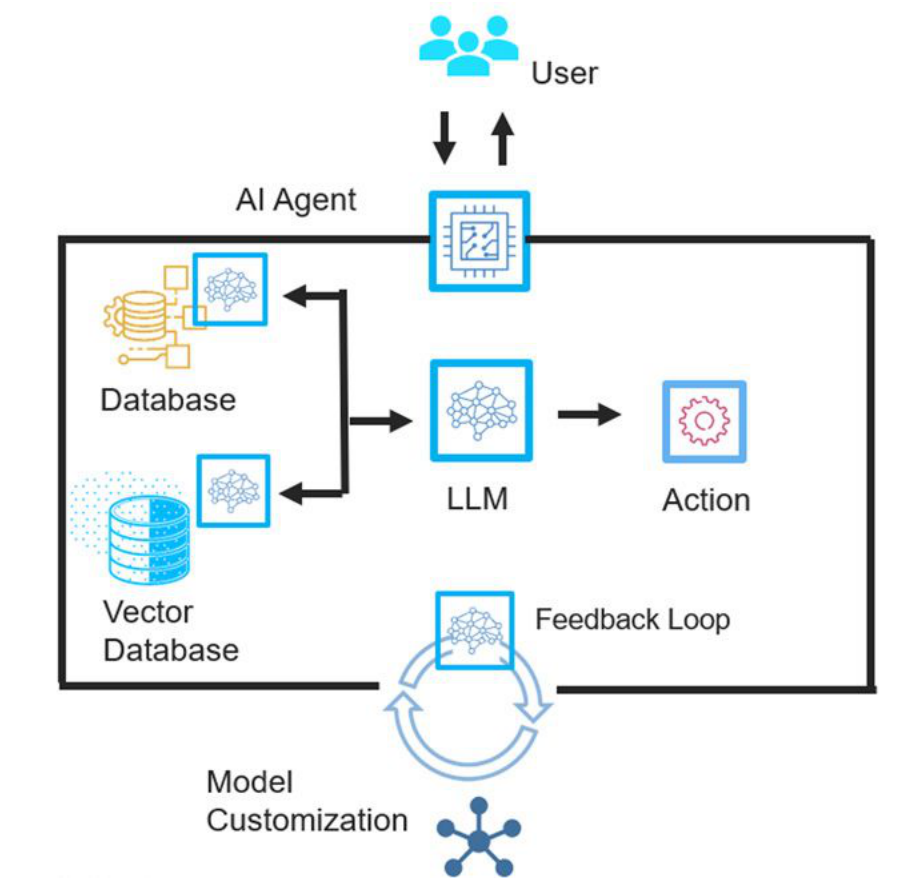
\includegraphics[width=0.98\textwidth, height=0.98\textheight, keepaspectratio]{images/multimodal-nlp-agentic-ai/agentic_ai_agent_components_diagram.png}
\end{frame}

\begin{frame}{What is Agentic AI?}
  \begin{itemize}
    \item[\textcolor{red}{$\triangleright$}] AI systems that \textbf{perceive, reason, plan,} and \textbf{act} to fulfill goals.
    \item[\textcolor{red}{$\triangleright$}] \textbf{Agent loop:} Observe $\rightarrow$ Plan $\rightarrow$ Act $\rightarrow$ Reflect $\rightarrow$ Learn
    \item[\textcolor{red}{$\triangleright$}] Inspired by cognitive science, robotics, and autonomous agents.
  \end{itemize}
  \vspace{1em}
  \textbf{Core Components:}
  \begin{itemize}
    \item[\textcolor{red}{$\triangleright$}] Memory
    \item[\textcolor{red}{$\triangleright$}] Planning
    \item[\textcolor{red}{$\triangleright$}] Tool-use (plugins, APIs)
    \item[\textcolor{red}{$\triangleright$}] Feedback-driven behavior
  \end{itemize}
\end{frame}

\begin{frame}{What is Agentic AI?}
  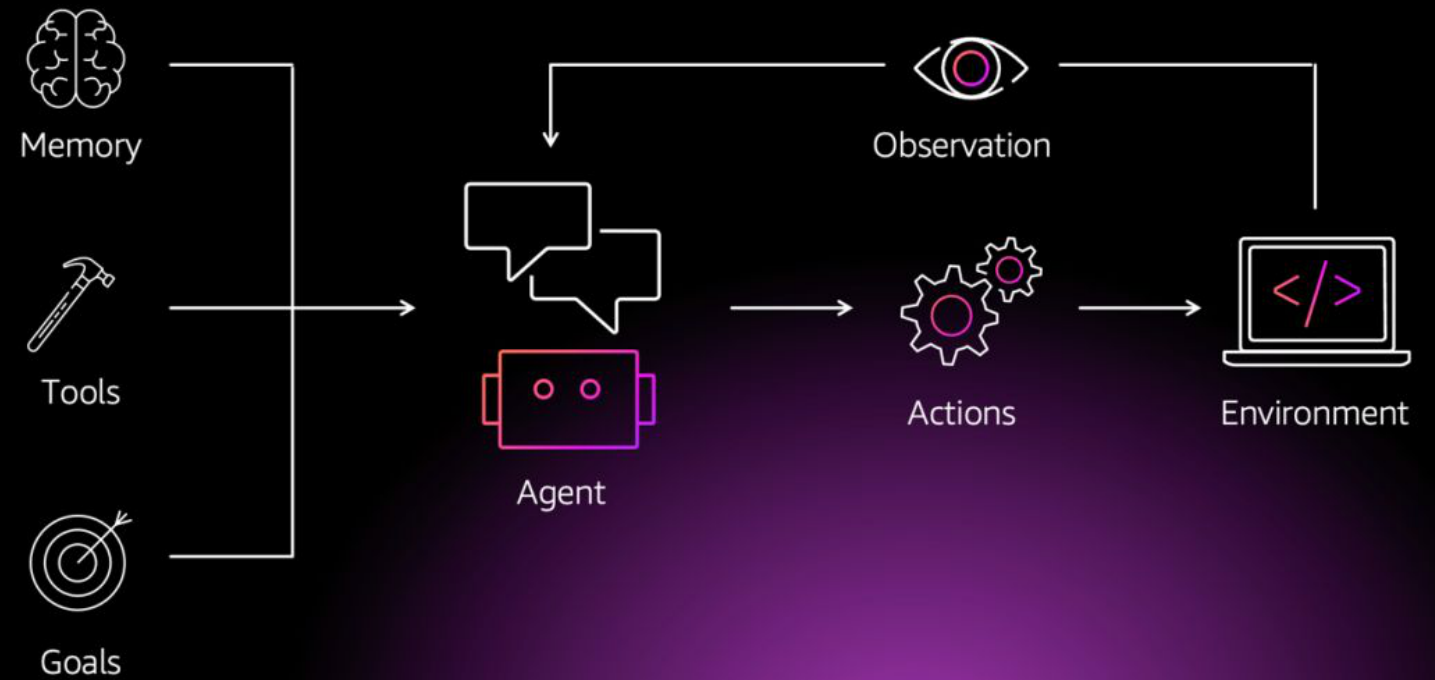
\includegraphics[width=0.98\textwidth, height=0.98\textheight, keepaspectratio]{images/multimodal-nlp-agentic-ai/agentic_agent_loop_memory_tools_goals.png}
\end{frame}

\begin{frame}{Reactive vs. Proactive Agents}
  \begin{table}[h!]
    \centering
    \begin{tabular}{l l l}
      \textbf{Feature} & \textbf{Reactive} & \textbf{Proactive} \\
      \hline
      Response & Immediate & Goal-oriented \\
      Planning & None & Yes \\
      Learning & Event-triggered & Self-initiated \\
      Example & Chatbots & Auto-GPT, Personal Assistants \\
    \end{tabular}
  \end{table}
  \vspace{1em}
  \textbf{Proactive agents} generate goals, schedule actions, and evaluate results even without user prompts.
\end{frame}

\begin{frame}{Reactive vs. Proactive Agents}
    \centering
    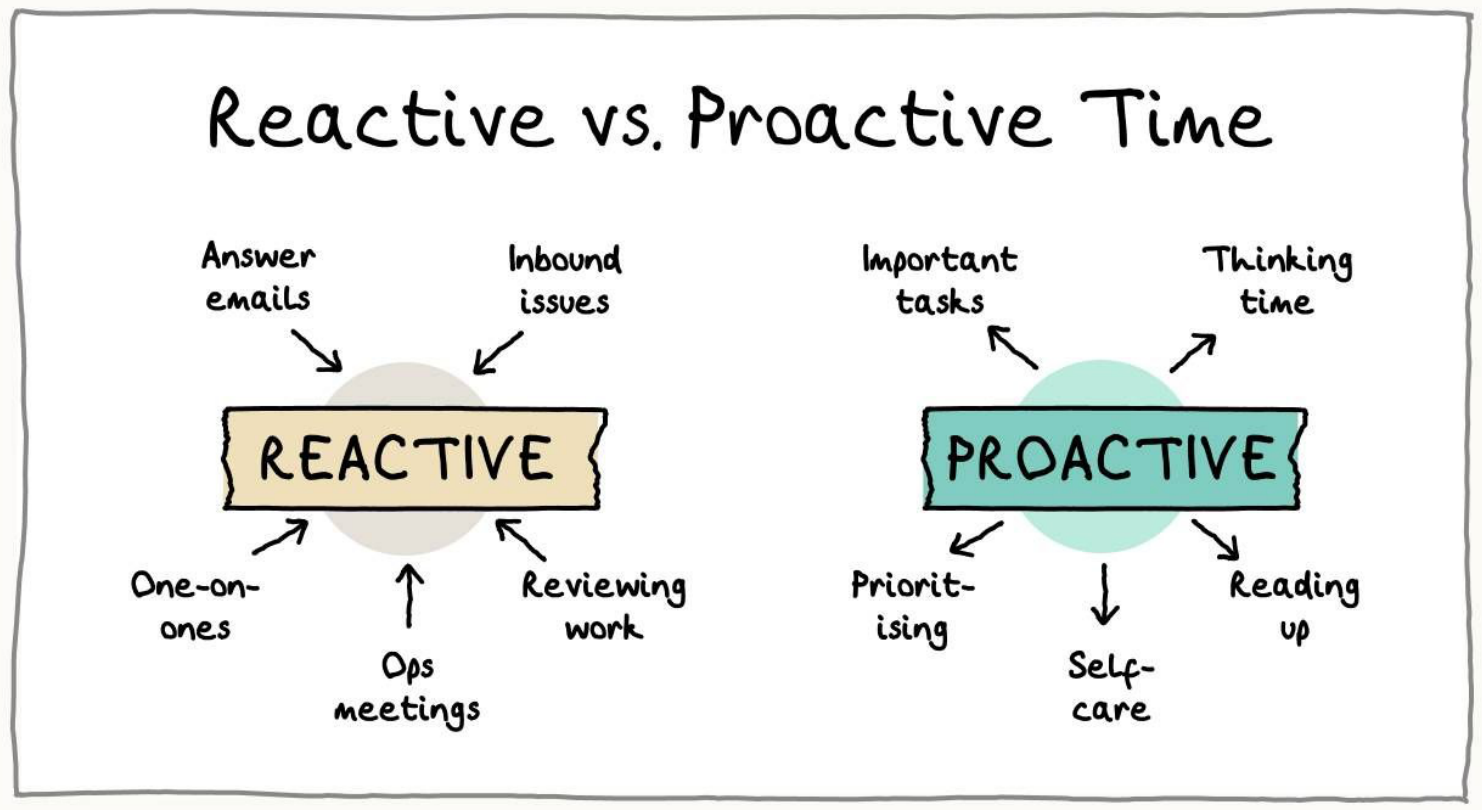
\includegraphics[width=0.98\textwidth, height=0.98\textheight, keepaspectratio]{images/multimodal-nlp-agentic-ai/agentic_reactive_vs_proactive_time.png}
\end{frame}

\begin{frame}{Reactive vs. Deliberative Agents}
  \centering
  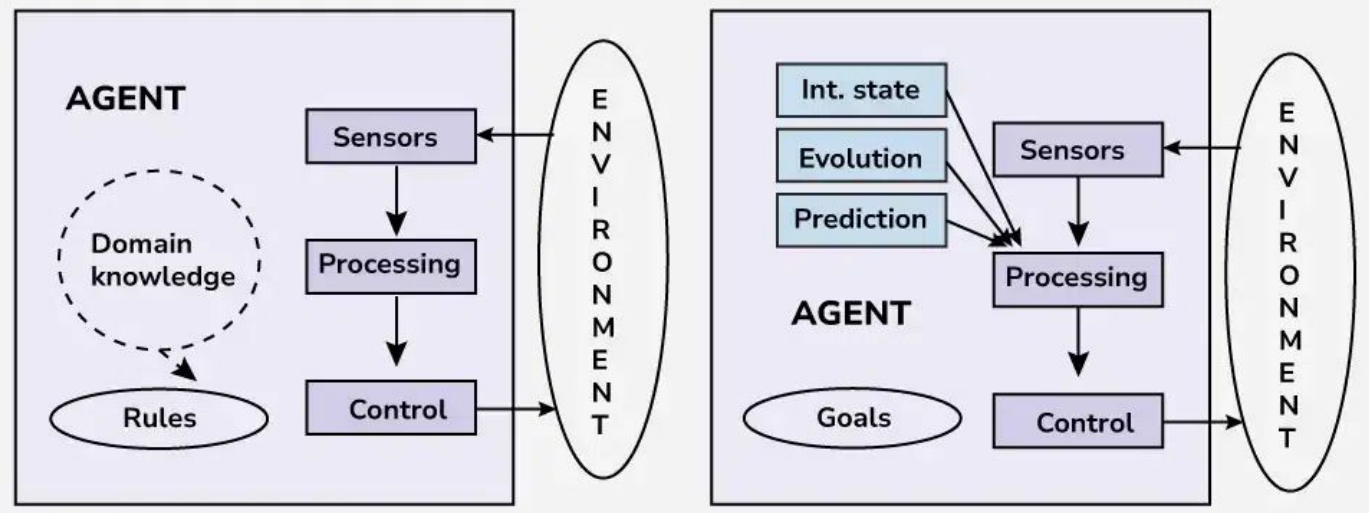
\includegraphics[width=0.98\textwidth, height=0.98\textheight, keepaspectratio]{images/multimodal-nlp-agentic-ai/agentic_reactive_vs_deliberative_agents.png}
\end{frame}

\begin{frame}{Reactive vs. Proactive Agents}
  \centering
  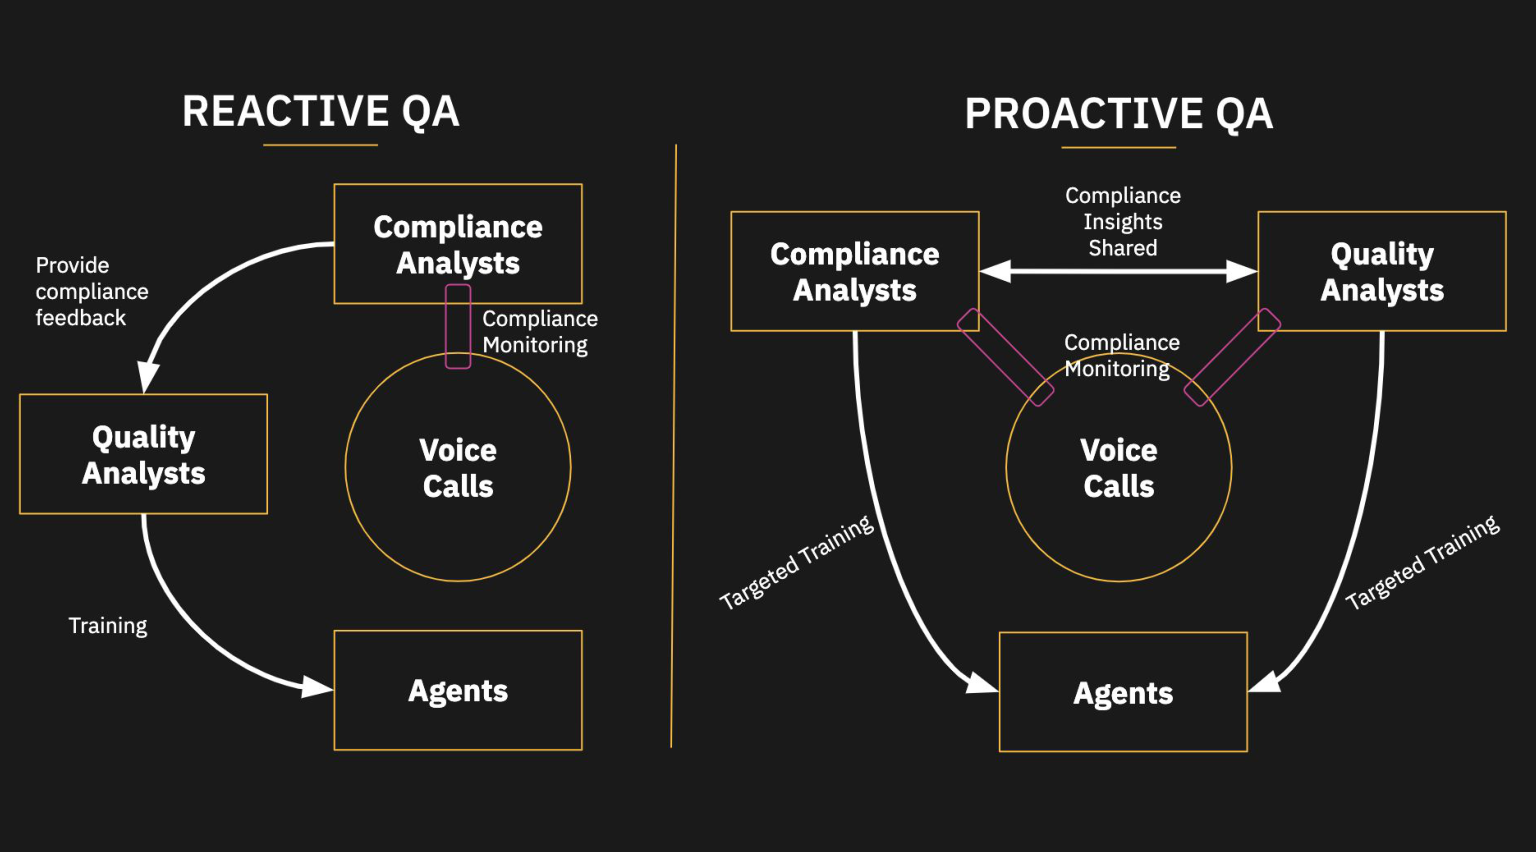
\includegraphics[width=0.98\textwidth, height=0.98\textheight, keepaspectratio]{images/multimodal-nlp-agentic-ai/agentic_reactive_vs_proactive_qa.png}
\end{frame}

\begin{frame}{Agent Loop in Detail}
  \textbf{\textcolor{red}{\large $\triangleright$ Perceive:}}~Multimodal input (text, vision, memory) \\
  \textbf{\textcolor{red}{\large $\triangleright$ Interpret:}}~NLP/vision models \\
  \textbf{\textcolor{red}{\large $\triangleright$ Plan:}}~Task decomposition (e.g., LangChain chains) \\
  \textbf{\textcolor{red}{\large $\triangleright$ Act:}}~API/tool calling \\
  \textbf{\textcolor{red}{\large $\triangleright$ Reflect \& Learn:}}~Refine memory or adjust goals
  \vspace{1em}
  
  \textbf{Applications:}
  \begin{itemize}
    \item[\textcolor{red}{$\triangleright$}] Personal AI assistants
    \item[\textcolor{red}{$\triangleright$}] Research co-pilots
    \item[\textcolor{red}{$\triangleright$}] Automated workflows
  \end{itemize}
\end{frame}

\begin{frame}{Tool Use and Function Calling}
  \begin{itemize}
    \item[\textcolor{red}{$\triangleright$}] \textbf{Function calling} is how an LLM acts: each tool is described to the model as a function with a name, a description, and a JSON schema for its parameters.
    \item[\textcolor{red}{$\triangleright$}] The model does not execute anything. It emits a structured call (function name + arguments); the runtime executes it and feeds the result back as a new message.
    \item[\textcolor{red}{$\triangleright$}] \textbf{The loop:} model receives the task $\rightarrow$ emits a call $\rightarrow$ runtime returns the result $\rightarrow$ model reasons over it $\rightarrow$ another call or a final answer.
    \item[\textcolor{red}{$\triangleright$}] Modern APIs support \textbf{parallel calls} (several independent tools in one step) and \textbf{structured outputs} (forcing the reply itself into a schema).
  \end{itemize}
\end{frame}

\begin{frame}[fragile]{Function Calling: Example}
  \textbf{Tool definition given to the model:}
  \begin{lstlisting}[language=Python]
{"name": "get_weather",
 "description": "Current weather for a city",
 "parameters": {"type": "object",
   "properties": {"city": {"type": "string"}},
   "required": ["city"]}}
  \end{lstlisting}
  \textbf{User:} ``Do I need an umbrella in Jeddah today?''
  \begin{lstlisting}[language=Python]
Model  -> call: get_weather(city="Jeddah")
Runtime-> result: {"condition": "rain", "temp_c": 24}
Model  -> "Yes, take one: it is raining in Jeddah (24 C)."
  \end{lstlisting}
\end{frame}

\begin{frame}{Agentic RAG}
  \begin{itemize}
    \item[\textcolor{red}{$\triangleright$}] \textbf{Fixed RAG pipeline:} retrieve once for the raw query, then generate. Fails when the query is vague, multi-part, or needs information the first retrieval missed.
    \item[\textcolor{red}{$\triangleright$}] \textbf{Agentic RAG} makes retrieval a tool the model controls:
    \begin{itemize}
      \item \textbf{Decide when:} answer directly from parametric knowledge, or retrieve.
      \item \textbf{Rewrite the query:} decompose multi-part questions into targeted searches.
      \item \textbf{Iterate:} retrieve, read, notice what is missing, retrieve again.
      \item \textbf{Judge the evidence:} discard irrelevant passages before answering.
    \end{itemize}
    \item[\textcolor{red}{$\triangleright$}] Costs more latency and tokens per query; pays off on multi-hop questions and heterogeneous document collections.
  \end{itemize}
\end{frame}

\begin{frame}{Agentic RAG Workflow}
  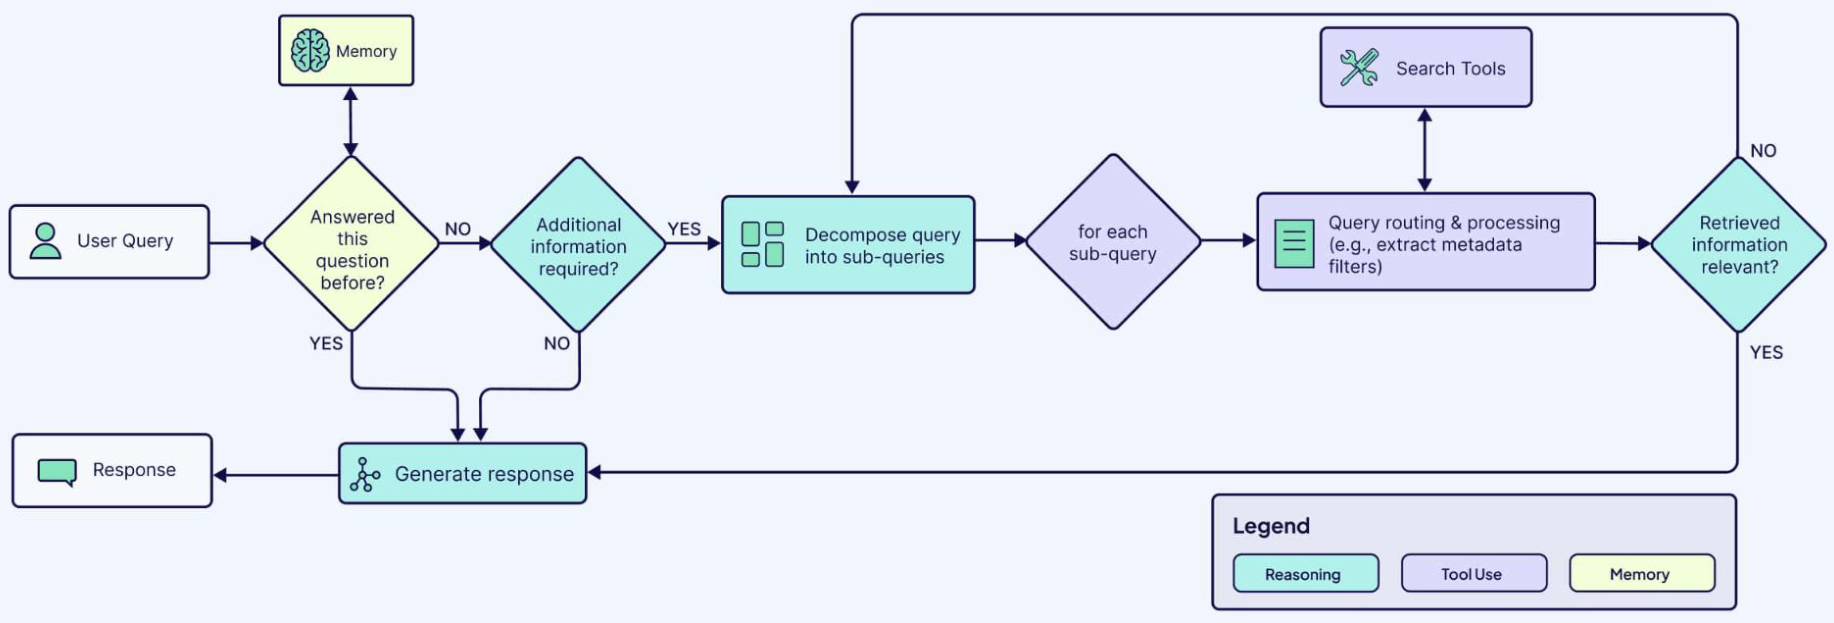
\includegraphics[width=0.98\textwidth, height=0.98\textheight, keepaspectratio]{images/multimodal-nlp-agentic-ai/agentic_rag_reasoning_flow.png}
\end{frame}

\begin{frame}{Open-Source Agentic Frameworks}
  \centering
  \Huge Open-Source Agentic Frameworks
\end{frame}

\begin{frame}{Auto-GPT}
  \centering
  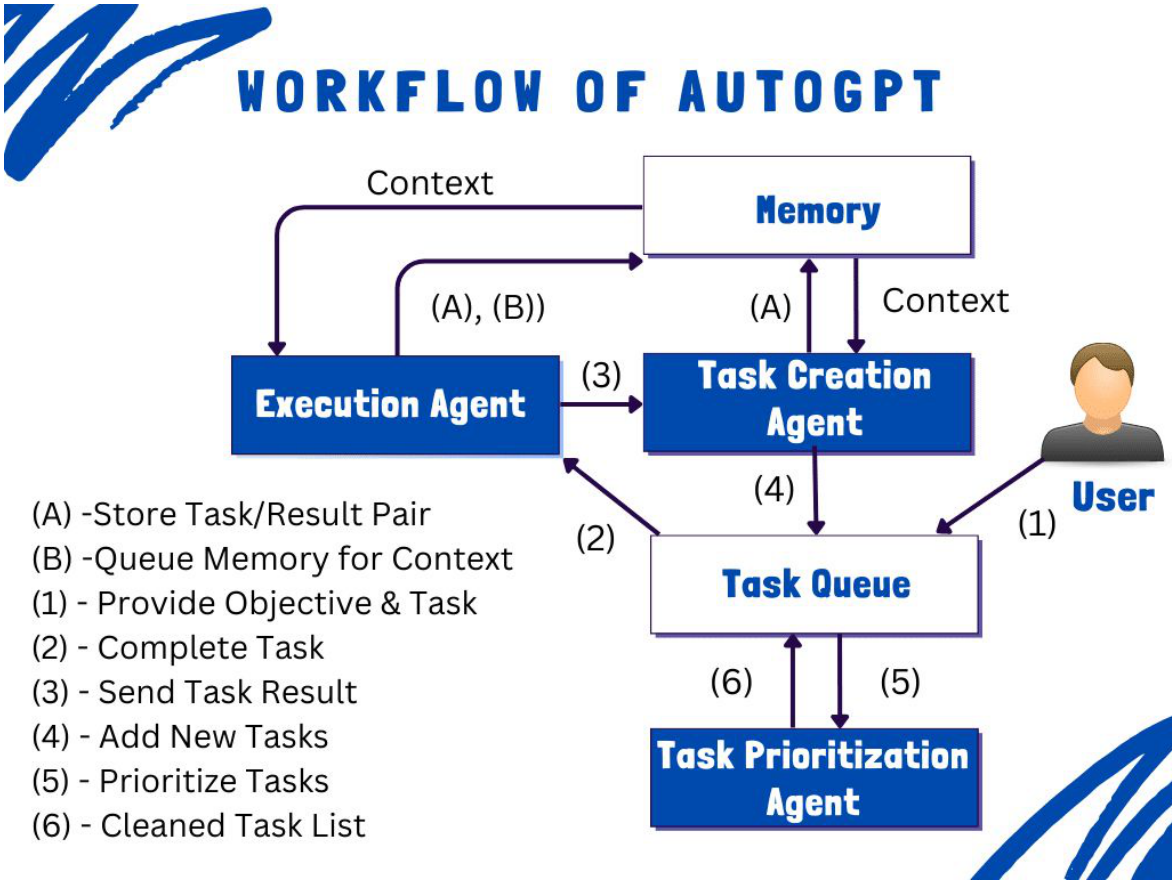
\includegraphics[width=0.98\textwidth, height=0.98\textheight, keepaspectratio]{images/multimodal-nlp-agentic-ai/agentic_autogpt_workflow.png}
\end{frame}

\begin{frame}{Auto-GPT}
    \textbf{Auto-GPT} is an \textbf{open-source project} that chains GPT calls to build autonomous agents.
    \begin{itemize}
        \item[\textcolor{red}{$\triangleright$}] \textbf{Open-source project} that chains GPT calls to build autonomous agents.
        \item[\textcolor{red}{$\triangleright$}] Uses \textbf{long-term memory}, file storage, and self-generated tasks.
        \item[\textcolor{red}{$\triangleright$}] \textbf{Requirements:}
        \begin{itemize}
            \item Task input
            \item Internet / API access
            \item Feedback loop
        \end{itemize}
    \end{itemize}
    \vspace{0.5em}
    \textbf{GitHub:} \href{https://github.com/Torantulino/Auto-GPT}{https://github.com/Torantulino/Auto-GPT}
\end{frame}

\begin{frame}{Auto-GPT}
  \centering
  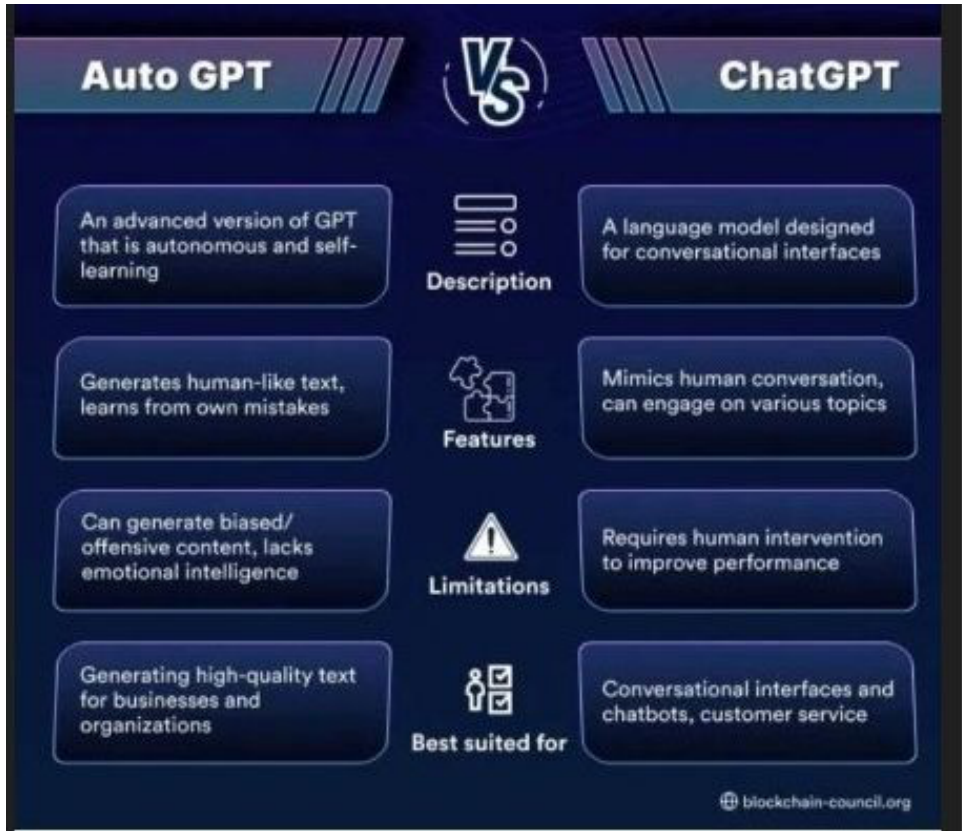
\includegraphics[width=0.98\textwidth, height=0.98\textheight, keepaspectratio]{images/multimodal-nlp-agentic-ai/agentic_autogpt_vs_chatgpt.png}
\end{frame}

\begin{frame}{BabyAGI}
  \centering
  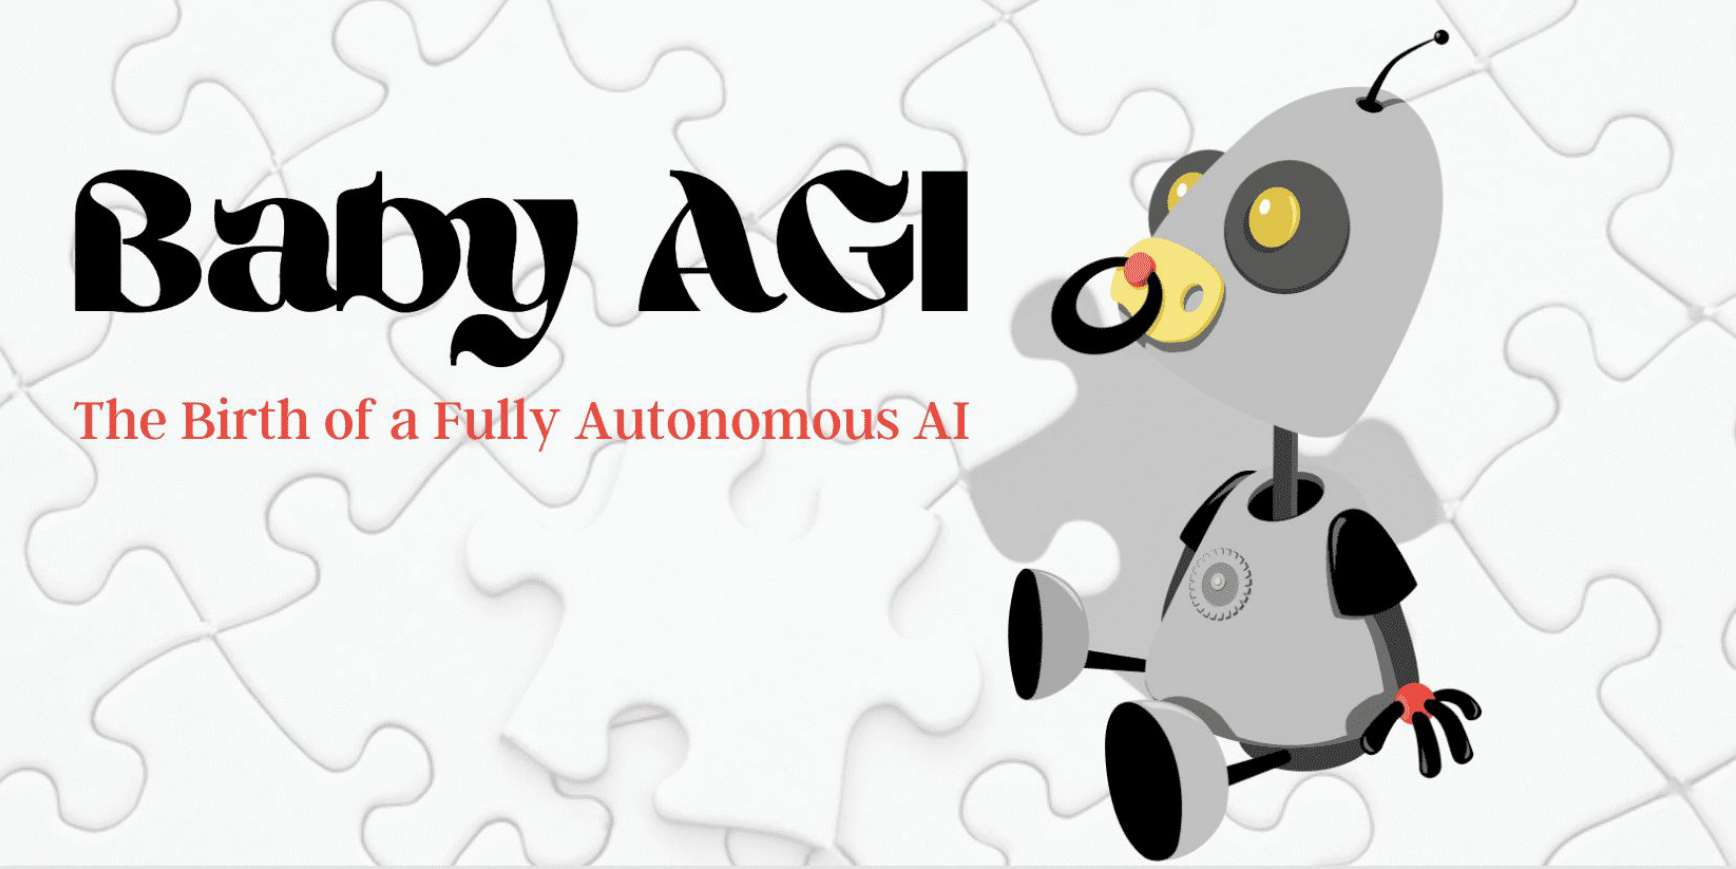
\includegraphics[width=0.98\textwidth, height=0.98\textheight, keepaspectratio]{images/multimodal-nlp-agentic-ai/agentic_babyagi_title.png}
\end{frame}

\begin{frame}{BabyAGI}
    \begin{itemize}
        \item[\textcolor{red}{$\triangleright$}] \textbf{Lightweight Python agent loop}
        \item[\textcolor{red}{$\triangleright$}] Generates tasks from high-level objectives
        \item[\textcolor{red}{$\triangleright$}] Runs tasks, stores results, and generates new tasks iteratively
        \item[\textcolor{red}{$\triangleright$}] Emphasizes simplicity and minimalism
    \end{itemize}
    \vspace{0.5em}
    \textbf{GitHub:} \href{https://github.com/yoheinakajima/babyagi}{https://github.com/yoheinakajima/babyagi}
\end{frame}


\begin{frame}{BabyAGI: How BabyAGI Works}
  \centering
  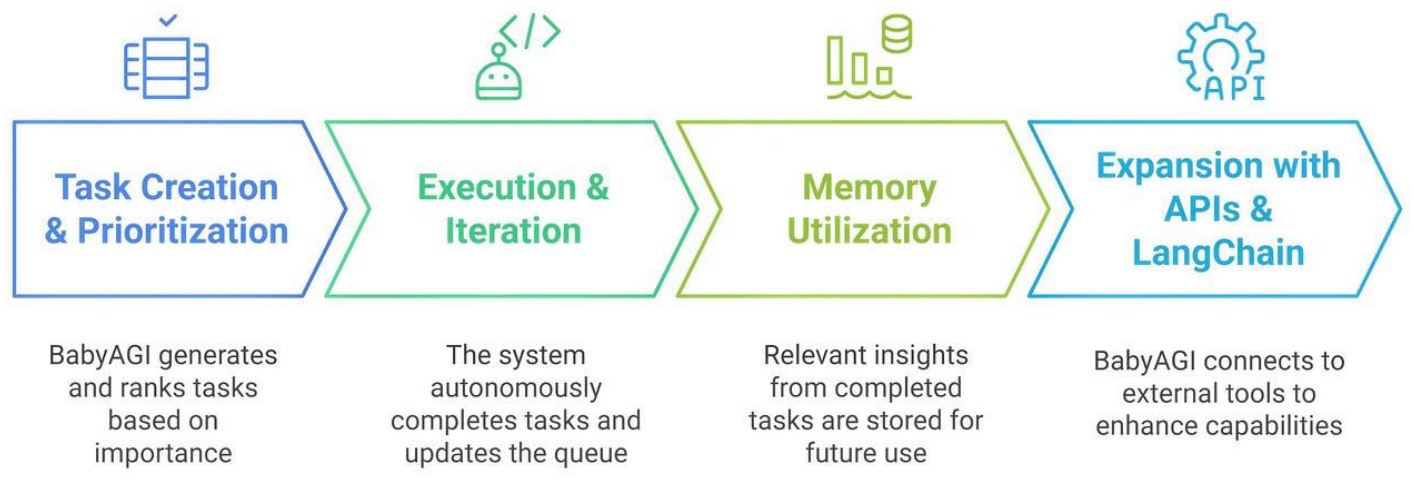
\includegraphics[width=0.98\textwidth, height=0.98\textheight, keepaspectratio]{images/multimodal-nlp-agentic-ai/agentic_babyagi_workflow_stages.png}
\end{frame}

\begin{frame}{Other Notable Frameworks}
  \begin{itemize}
    \item[\textcolor{red}{$\triangleright$}] \textbf{LangChain:} Framework for chaining LLMs with tools, APIs, and memory. Enables complex workflows and agentic behavior.
    \item[\textcolor{red}{$\triangleright$}] \textbf{CrewAI:} Multi-agent coordination platform for collaborative task execution.
    \item[\textcolor{red}{$\triangleright$}] \textbf{SuperAGI:} Production-grade agent platform supporting extensibility, monitoring, and deployment.
    \item[\textcolor{red}{$\triangleright$}] \textbf{OpenDevin:} Developer-oriented agentic IDE for automating software engineering tasks.
  \end{itemize}
\end{frame}

\begin{frame}{LangChain}
  \centering
  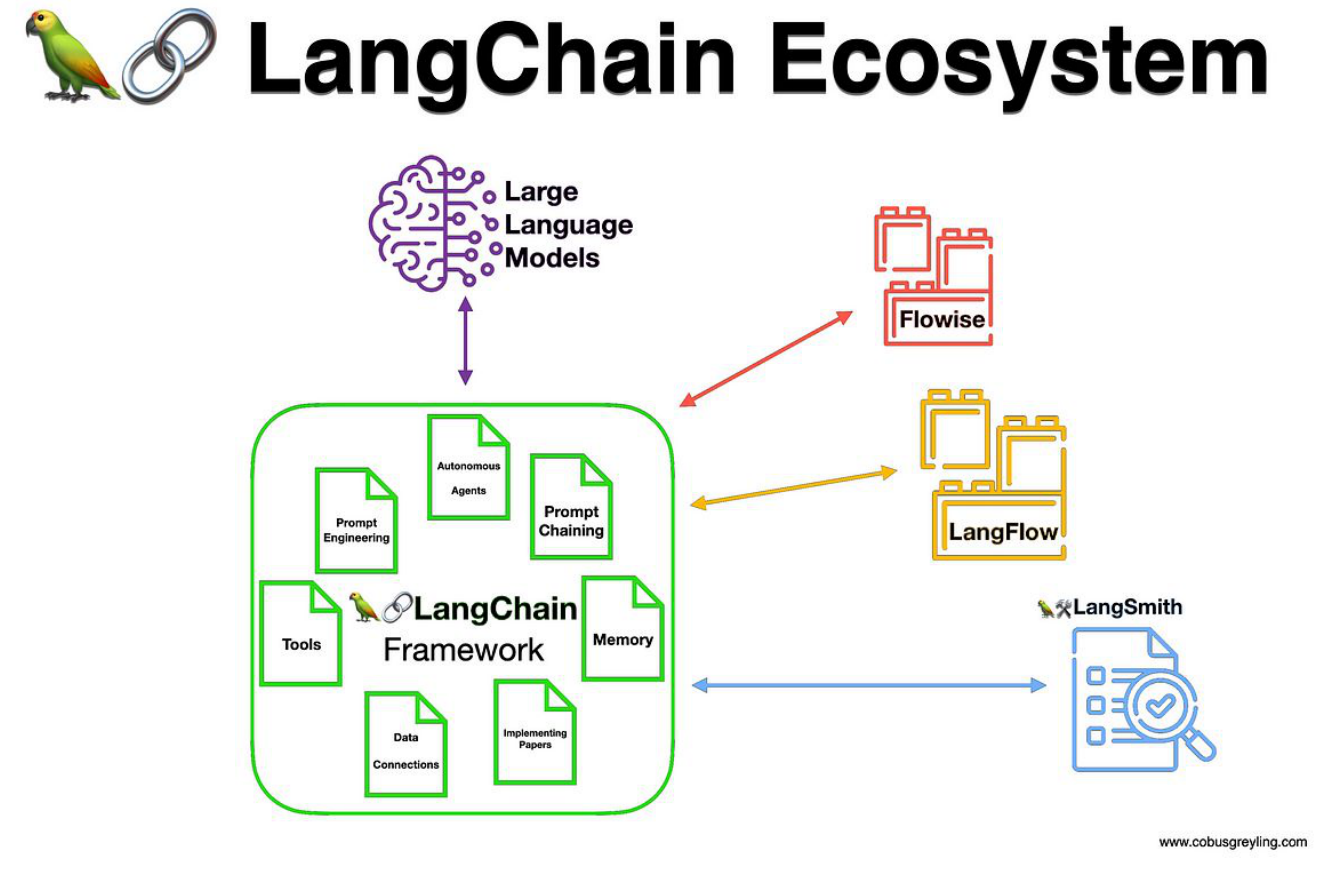
\includegraphics[width=0.98\textwidth, height=0.98\textheight, keepaspectratio]{images/multimodal-nlp-agentic-ai/agentic_langchain_ecosystem.png}
\end{frame}

\begin{frame}{CrewAI}
  \centering
  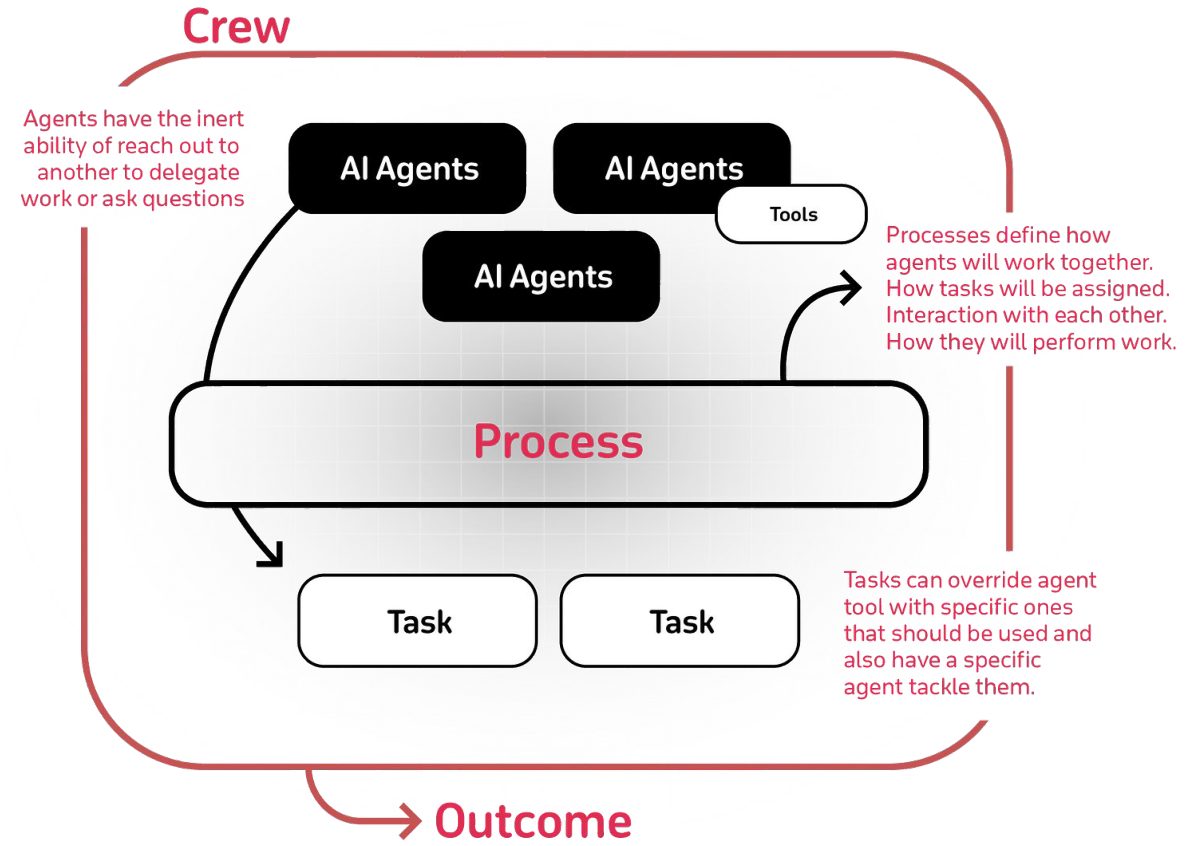
\includegraphics[width=0.98\textwidth, height=0.98\textheight, keepaspectratio]{images/multimodal-nlp-agentic-ai/agentic_crewai_process_diagram.png}
\end{frame}

\begin{frame}{SuperAGI}
  \centering
  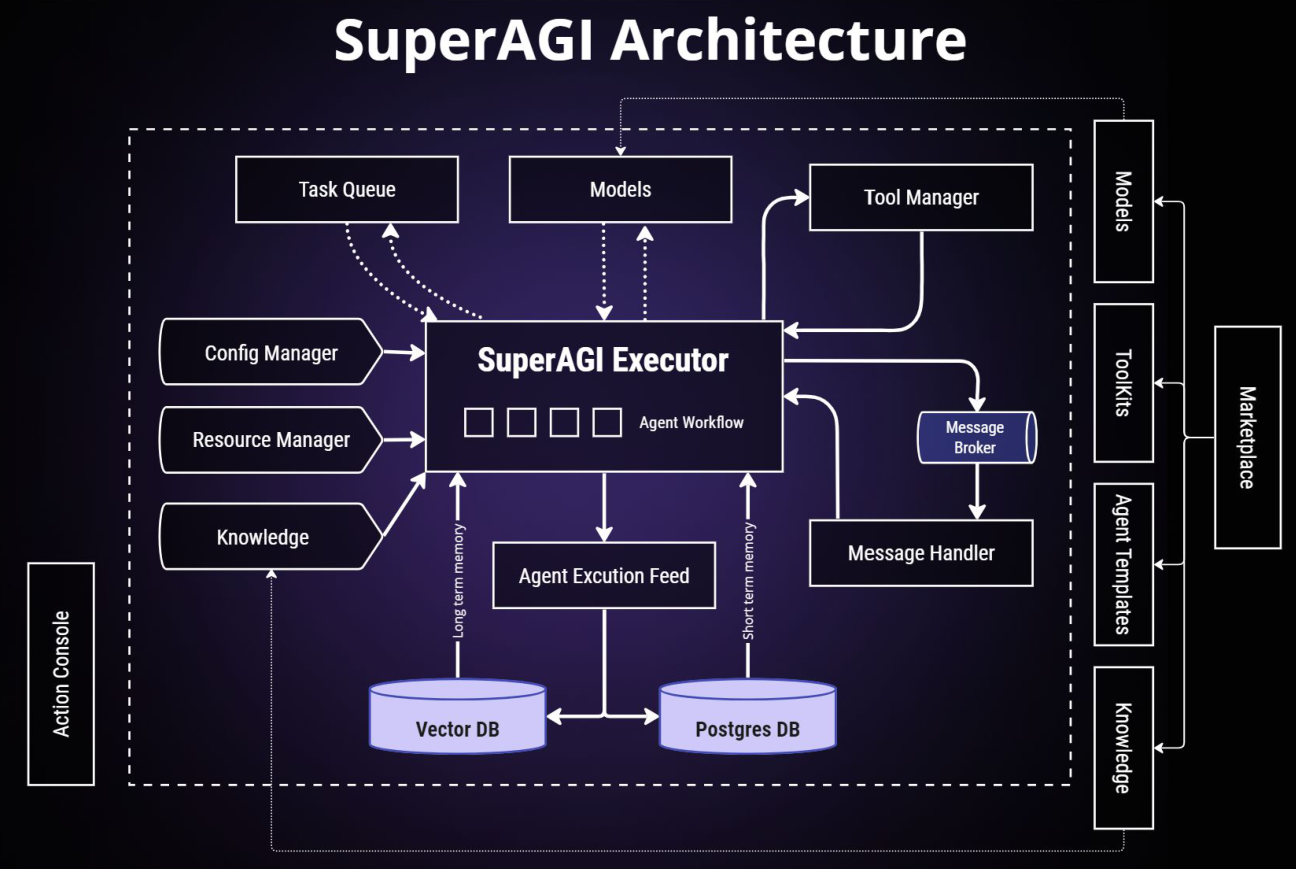
\includegraphics[width=0.98\textwidth, height=0.98\textheight, keepaspectratio]{images/multimodal-nlp-agentic-ai/agentic_superagi_architecture.png}
\end{frame}

\begin{frame}{SuperAGI}
  \centering
  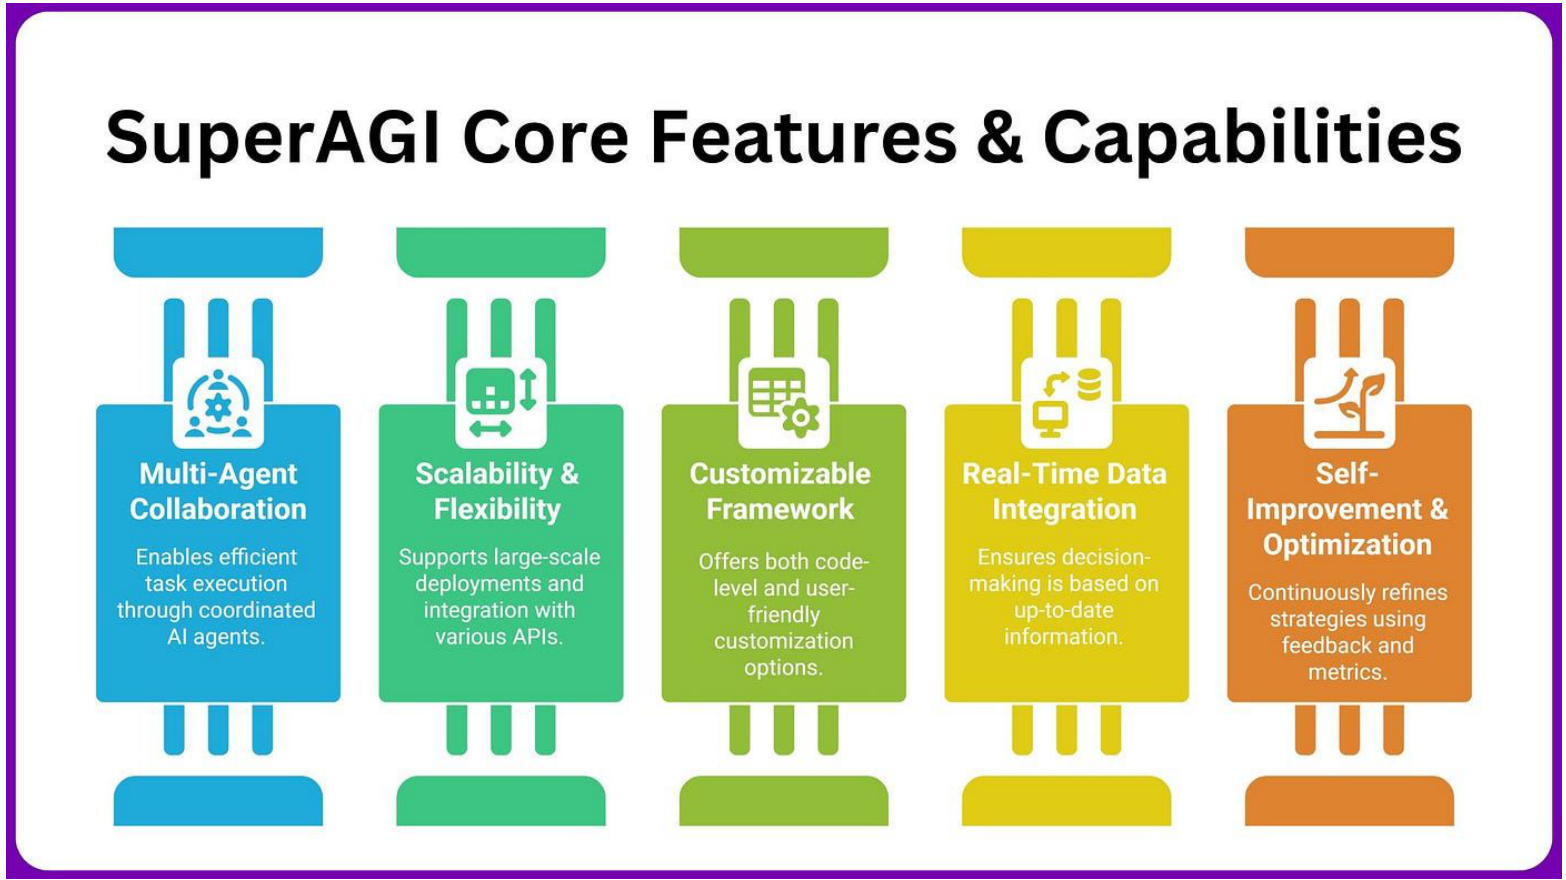
\includegraphics[width=0.98\textwidth, height=0.98\textheight, keepaspectratio]{images/multimodal-nlp-agentic-ai/agentic_superagi_core_features.png}
\end{frame}

\begin{frame}{OpenDevin}
  \centering
  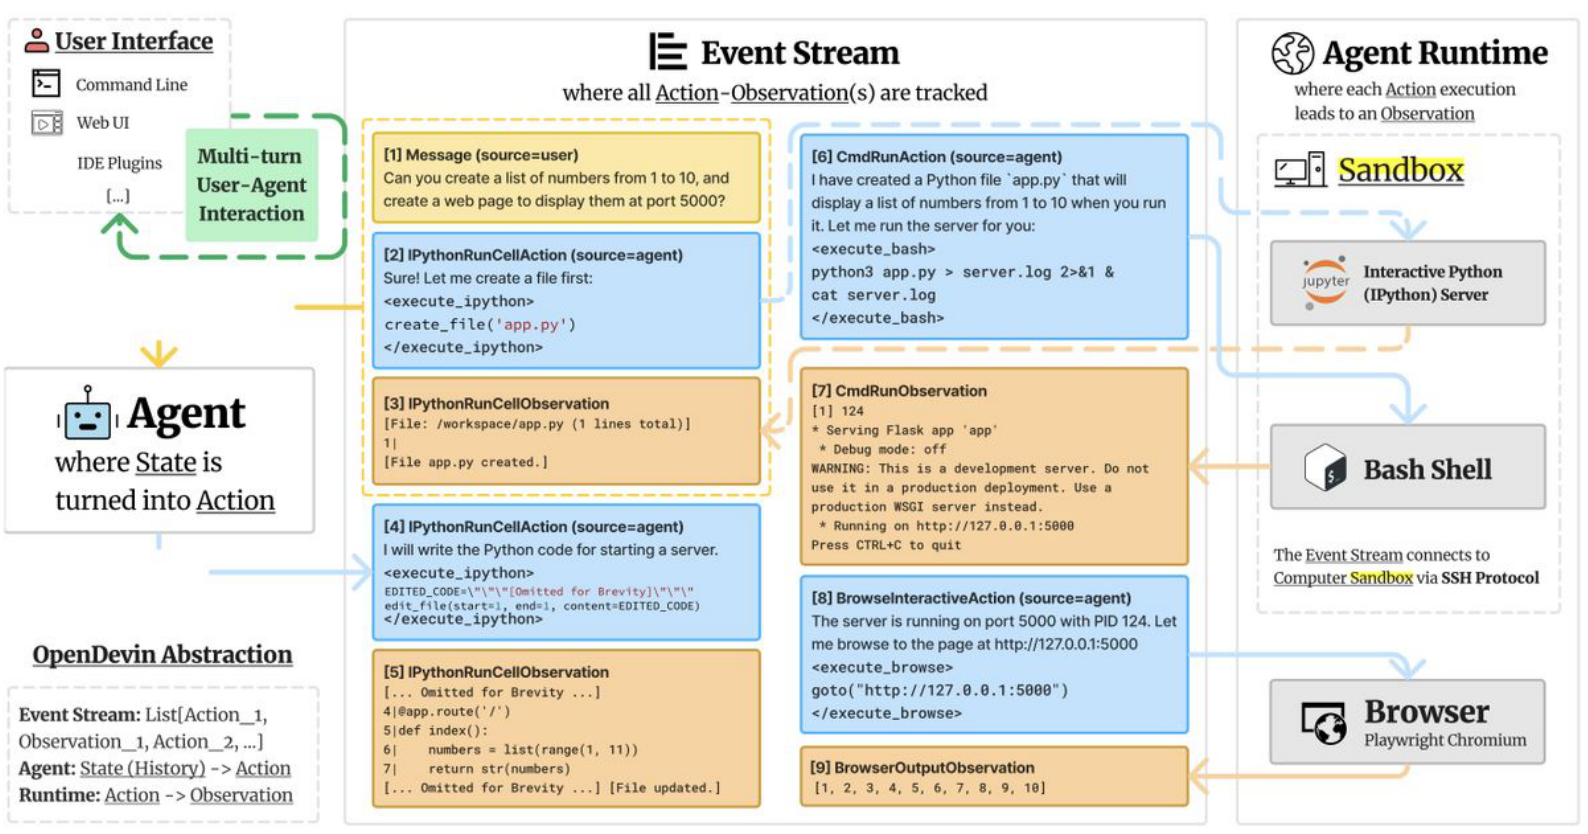
\includegraphics[width=0.98\textwidth, height=0.98\textheight, keepaspectratio]{images/multimodal-nlp-agentic-ai/agentic_opendevin_event_stream.png}
\end{frame}
